\section{Method}\label{sec:method}

We describe the model configurations, evaluation benchmarks, and analytical framework used to measure how attention affects cross-architecture agreement at both aggregate and per-example levels.

\begin{table}[t]
\centering
\small
\caption{Model zoo summary \citep{wang2025hybrid}. All configurations share training data, tokenizer, and hyperparameters; they differ only in backbone and attention ratio.}
\label{tab:model_zoo}
\begin{tabular}{@{}lll@{}}
\toprule
Architecture & Recurrence mechanism & Scales \\
\midrule
GatedDeltaNet & Gated delta rules & 340M, 1.3B \\
RetNet & Multi-scale exp.\ decay & 340M, 1.3B \\
HGRN2 & Gated state expansion & 340M, 1.3B \\
\midrule
\multicolumn{3}{@{}l@{}}{\footnotesize Attention ratios: 0\%, 4\%, 7.7\%, 14.3\%, 25\%} \\
\multicolumn{3}{@{}l@{}}{\footnotesize Extended (340M only): +GLA, +DeltaNet} \\
\bottomrule
\end{tabular}
\end{table}

\subsection{Model Zoo}\label{ssec:model_zoo}

We use the pretrained model zoo of \citet{wang2025hybrid} (Table~\ref{tab:model_zoo}), which provides controlled comparisons: GatedDeltaNet (GDN; \citealp{yang2024gateddeltanet}), RetNet \citep{sun2023retnet}, and HGRN2 \citep{qin2024hgrn2} at five attention ratios and two scales. The GDN 1.3B h3-1 configuration uses 16 attention heads vs.\ 32 for RetNet and HGRN2 (\S\ref{ssec:robustness}). We adopt the h$k$-1 notation: h3-1 = 25\% attention, h6-1 = 14.3\%, h12-1 = 7.7\%, h24-1 = 4\%. Within each scale, all models share identical training data, tokenizer, and hyperparameters, isolating architecture and attention configuration. The zoo also includes a Transformer baseline at both scales.

\subsection{Task Taxonomy}\label{ssec:task_taxonomy}

We evaluate on 10 benchmarks grouped into four categories defined by the primary cognitive demand of each task. This taxonomy (informal; not pre-registered) was fixed prior to analysis following standard categorizations in the evaluation literature \citep{arora2024zoology} and is treated as hypothesis-generating rather than confirmatory (see Appendix~\ref{app:benchmark_details} for the confirmatory/exploratory split), not derived post hoc from observed results. The categories test whether the effect of attention on cross-architecture variance depends on task type.

\begin{itemize}
    \item \textbf{Retrieval}: LAMBADA \citep{paperno2016lambada}, which requires predicting a final word from long-range context without reasoning or world knowledge.
    \item \textbf{Comprehension}: BoolQ \citep{clark2019boolq}, a reading comprehension task with yes/no answers.
    \item \textbf{Reasoning}: HellaSwag \citep{zellers2019hellaswag}, ARC-Challenge \citep{clark2018arc}, WinoGrande \citep{sakaguchi2020winogrande}, and PIQA \citep{bisk2020piqa}. COPA \citep{roemmele2011copa} ($n = 100$) is supplementary; its small sample renders $\alpha$ unreliable (Appendix~\ref{app:subsample_sensitivity}).
    \item \textbf{Mixed}: ARC-Easy \citep{clark2018arc}, MMLU \citep{hendrycks2021mmlu}, SciQ \citep{welbl2017sciq}, and XStoryCloze \citep{lin2022xstorycloze}, which combine retrieval, comprehension, and reasoning demands.
\end{itemize}

LAMBADA is the only free-form generation benchmark in our evaluation; all others use multiple-choice scoring. Its higher $\alpha$ (0.30 vs.\ 0.14--0.21 for multiple-choice tasks) may partly reflect the larger answer space inherent to open-ended prediction, and the multiple-choice format may mechanically constrain per-example divergence by limiting the number of distinct error patterns. We cannot fully disentangle task type from evaluation format with the present benchmarks. However, within multiple-choice tasks, format (two-way vs.\ four-way) does not predict $\alpha$ (\S\ref{ssec:per_example}), suggesting that format alone does not drive the observed variation.

All evaluations use lm-evaluation-harness v0.4.x \citep{gao2024lmeval} with default prompts and greedy decoding; accuracy serves as the primary metric for all benchmarks. Bootstrap analyses use random seed 42 throughout.

\subsection{Convergence Metrics}\label{ssec:convergence_metrics}

We quantify cross-architecture agreement as a function of attention ratio. For each benchmark and attention ratio, we compute the cross-architecture standard deviation $\sigma$ over the three architectures' accuracy scores. To measure the relationship between attention and convergence, we compute the Spearman rank correlation $\rho$ between attention ratio rank and $\sigma$ across the five attention configurations ($n = 5$). A negative $\rho$ indicates that higher attention ratios are associated with lower cross-architecture variance.

We also report the convergence ratio $\sigma_{\text{pure}} / \sigma_{\text{h3-1}}$, defined as the standard deviation under the pure-recurrent configuration divided by that under the highest attention ratio (25\%). Values greater than 1 indicate that higher attention ratios are associated with lower cross-architecture variance.

\begin{figure}[t]
\centering
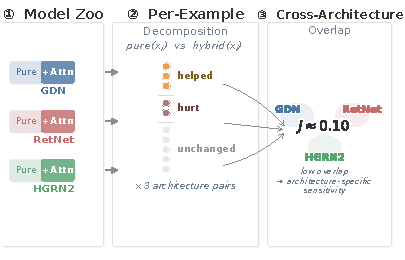
\includegraphics[width=\columnwidth]{figures/fig_method_overview.pdf}
\caption{Experimental framework. For each architecture, we compare the pure-recurrent baseline against its hybrid (+attention) variant, classifying every evaluation example as helped, hurt, or unchanged. Cross-architecture overlap of these per-example effect sets is measured via pairwise Jaccard similarity ($J \approx 0.10$), revealing architecture-specific sensitivity patterns.}
\label{fig:method_overview}
\end{figure}

\subsection{Per-Example Decomposition}\label{ssec:per_example_decomposition}

We decompose performance changes at the individual-example level on four benchmarks spanning three task categories: LAMBADA (5{,}153 examples; retrieval), HellaSwag (10{,}042; reasoning), PIQA (1{,}838; reasoning, two-choice), and ARC-Easy (2{,}376; mixed). HellaSwag uses normalized accuracy (acc\_norm) as the per-example correctness criterion. Supplementary analyses on BoolQ (3{,}270) and WinoGrande (1{,}267) appear in Appendix~\ref{app:boolq} and \ref{app:winogrande}. For each architecture, we compare the pure-recurrent baseline against its h3-1 hybrid (25\% attention), which maximizes the recurrent--hybrid contrast; \S\ref{ssec:per_example} confirms that $\alpha$ is stable across intermediate ratios (variation $< 0.03$). Each example is classified as:

\begin{itemize}
    \item \textbf{Helped}: correct in the hybrid but incorrect in the pure model.
    \item \textbf{Hurt}: correct in the pure model but incorrect in the hybrid.
    \item \textbf{Unchanged}: both models agree (both correct or both incorrect).
\end{itemize}

The net effect for each architecture is $|\text{helped}| - |\text{hurt}|$. A positive net effect means more examples transition to correct than to incorrect when attention is added; a negative net effect means the opposite.

To measure cross-architecture overlap, we compute the pairwise Jaccard similarity $J = |A \cap B| / |A \cup B|$ between the helped sets of two architectures and, separately, between their hurt sets. $J = 1$ indicates identical sets; $J = 0$ indicates no overlap. On $K$-choice tasks, binarization collapses $K{-}1$ wrong answers into a single ``incorrect'' category, potentially counting architectures as agreeing (both wrong) when they select different wrong answers. This conservative bias strengthens the multiplicity claim: true divergence may exceed what binary Jaccard captures. Appendix~\ref{app:continuous_jaccard} confirms robustness under continuous Jaccard similarity.

\subsection{Statistical Methods}\label{ssec:statistical_methods}

All tests are two-tailed. Spearman $\rho$ uses exact permutation tests ($5! = 120$ permutations); with $n = 5$, only $|\rho| = 1.0$ achieves $p < .05$ ($p = .017$), so all Spearman-based inferences are descriptive and exploratory. Bonferroni correction spans all 10 benchmarks (adjusted threshold $\alpha / 10 = 0.005$). Bootstrap 95\% bias-corrected and accelerated (BCa) confidence intervals use 10{,}000 resamples; with $n = 3$ architectures, these are heuristic indicators of effect direction. Within-architecture comparisons use Mann-Whitney U; cross-architecture comparisons use Kruskal-Wallis. Attention weight analysis extracts per-layer cosine similarity and Shannon entropy via forward hooks (Appendix~\ref{app:attention_patterns}). The permutation null does not condition on item difficulty; if difficulty-driven correlations inflate observed Jaccard while permutation destroys this structure, the test may be anti-conservative. However, the ${\sim}2\times$ observed-to-null ratio (all $z > 5.9$) provides substantial margin against this bias.

\begin{figure}[t]
\centering
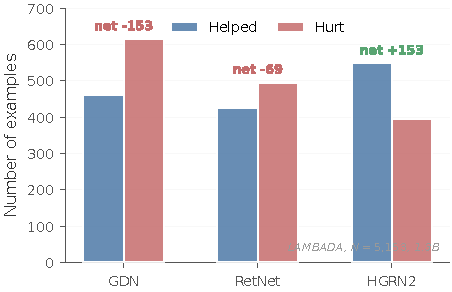
\includegraphics[width=\columnwidth]{figures/fig_per_example_bars.pdf}
\caption{Per-example effects of adding attention (pure $\to$ h3-1) on LAMBADA (1.3B). Helped: correct only with attention; hurt: correct only without. HGRN2 shows the only net positive effect; overlap is minimal ($\bar{J} \leq 0.10$, all $p < .0001$).}
\label{fig:per_example_bars}
\end{figure}
